\mode*

\section{Vad är en fil?}

\begin{frame}
  \begin{definition}[Primärminne]
    \begin{itemize}
      \item Datorns arbetsminne.
      \item Exekverande program (processer) och data (variabler) lagras här.
      \item Flyktigt minne.
    \end{itemize}
  \end{definition}

  \begin{definition}[Sekundärminne]
    \begin{itemize}
      \item Långsammare minne.
      \item Oflyktigt.
      \item Icke-exekverande program och data (filer) lagras här.
    \end{itemize}
  \end{definition}
\end{frame}

\begin{frame}
  \begin{block}{Filer}
    \begin{itemize}
      \item Vi har erfarenhet av filer.
      \item Våra program är sparade i filer.
    \end{itemize}
  \end{block}

  \pause

  \begin{example}
    \begin{itemize}
      \item Pythonprogram,
      \item bilder,
      \item Worddokument,
      \item \etc
    \end{itemize}
  \end{example}
\end{frame}

\begin{frame}
  \begin{remark}
    \begin{itemize}
      \item Behövs för att minnas mellan körningarna.
      \item Behövs för att överföra data mellan program.
      \item Behövs för att hantera kopiösa mängder data.
    \end{itemize}
  \end{remark}
\end{frame}


\section{Hur använder vi filer?}

\begin{frame}
  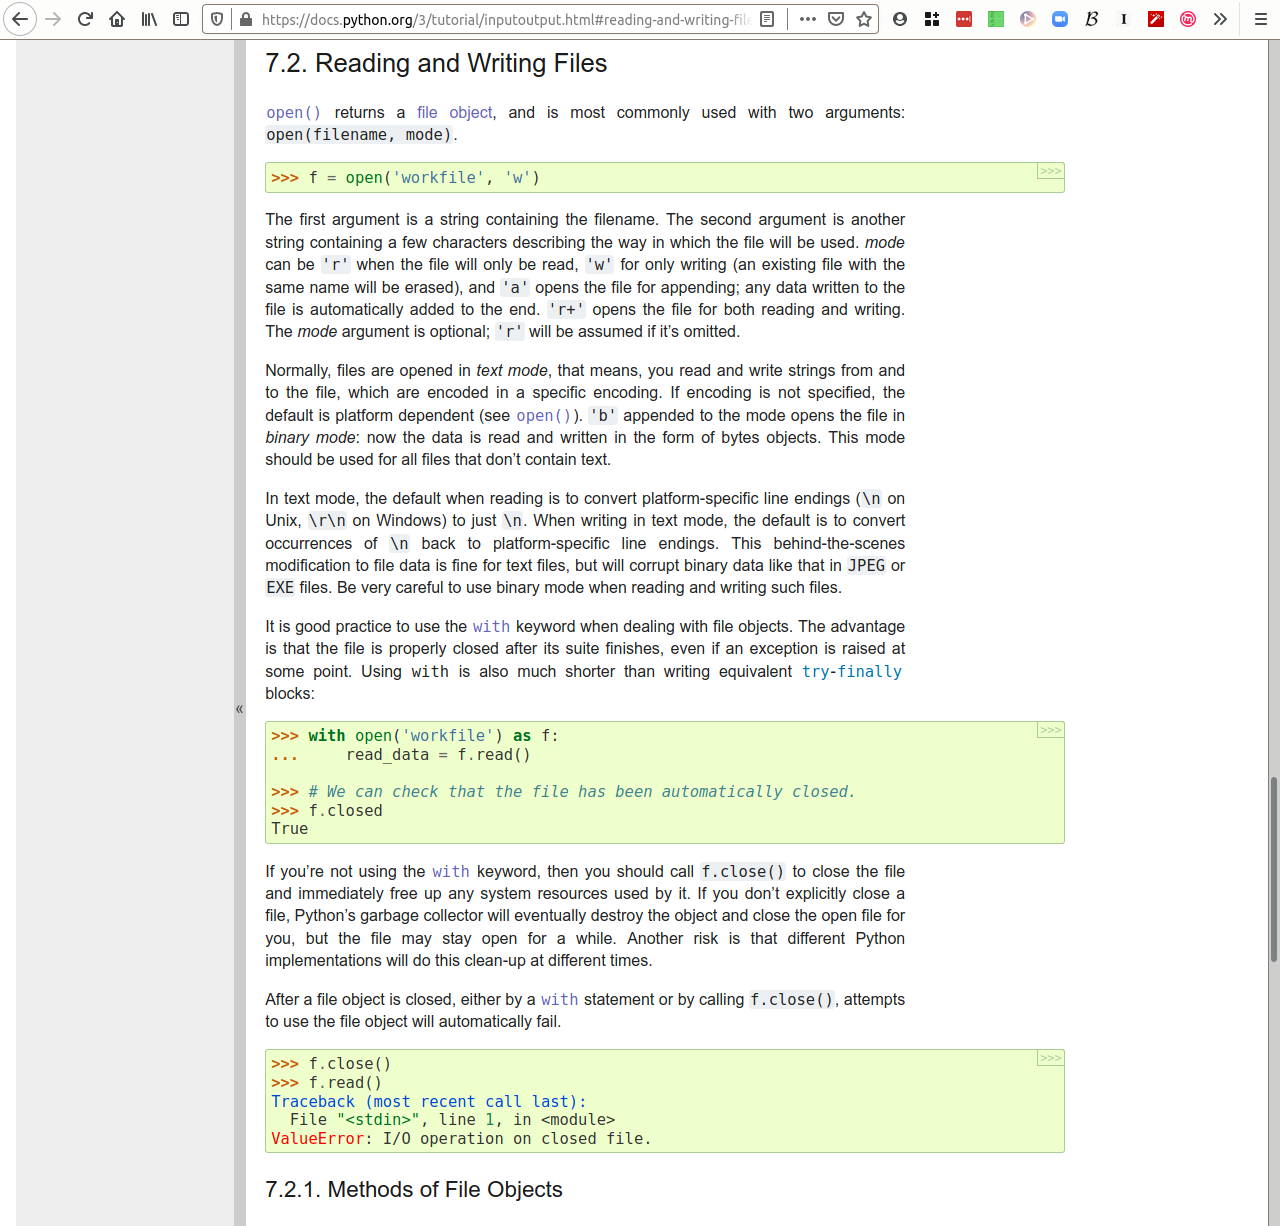
\includegraphics[width=\columnwidth]{figs/docs-files.png}
\end{frame}

\subsection{Öppna och stänga}

\begin{frame}[fragile]
  \begin{lstlisting}[numbers=none,basicstyle=\Large]
file = open("filename", "r")
print(file.read())
file.close()
  \end{lstlisting}
\end{frame}

\begin{frame}[fragile]
  \begin{example}[open\textunderscore close.py, del 1]
    \lstinputlisting[linerange=3-16,firstnumber=3]{examples/open_close.py}
  \end{example}
\end{frame}

\begin{frame}
  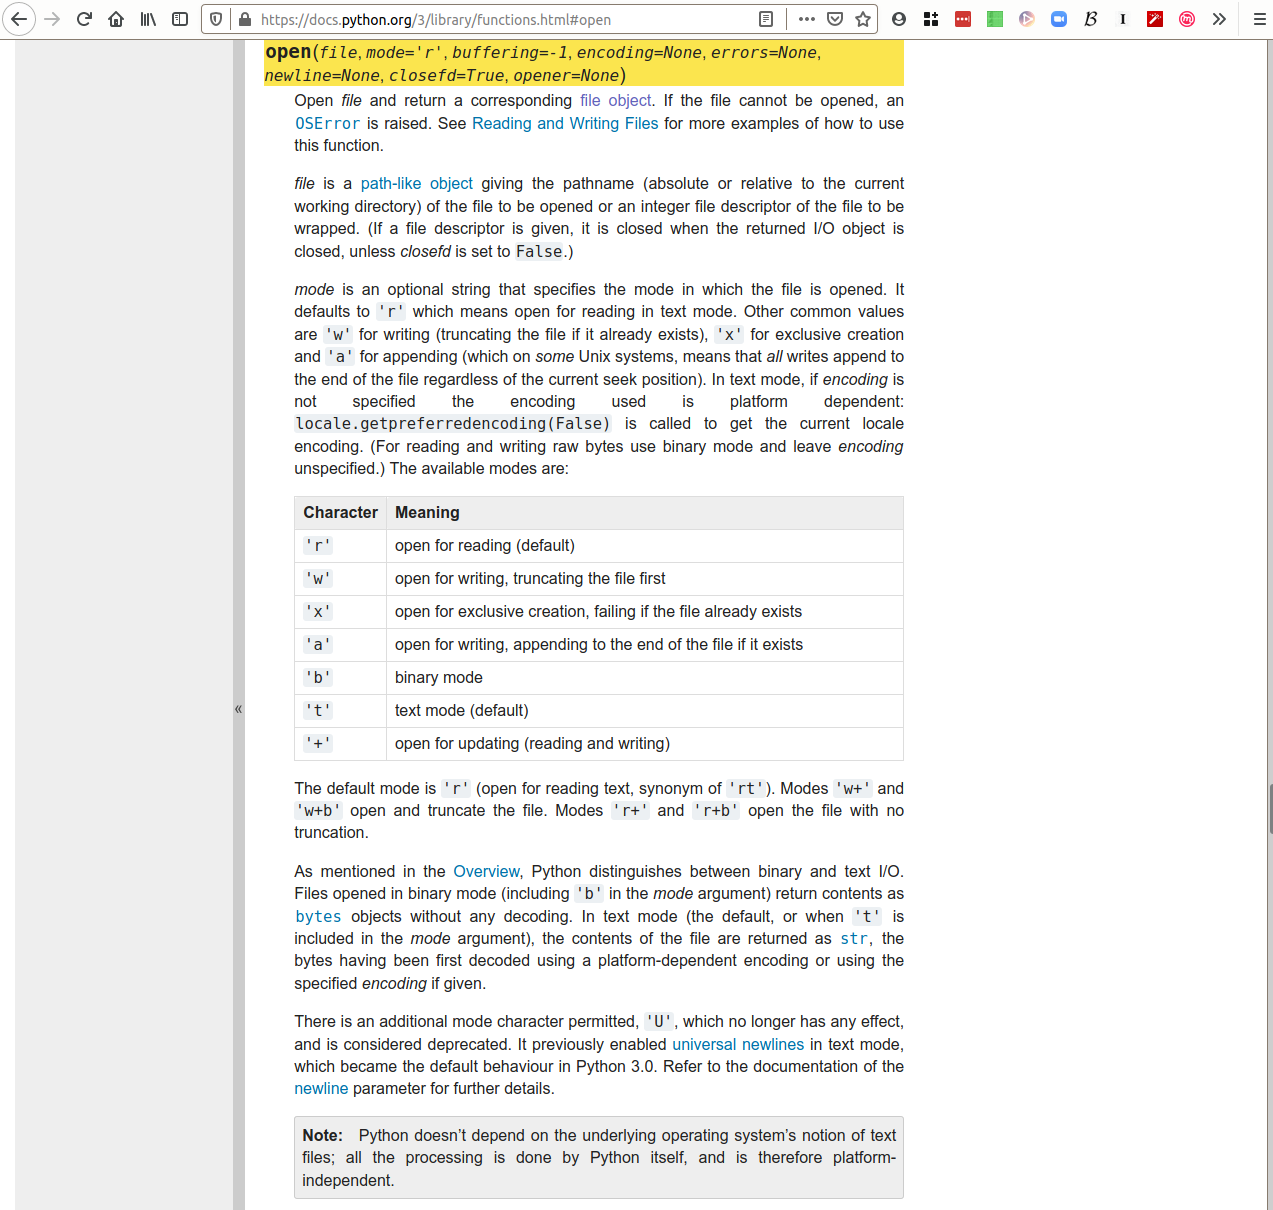
\includegraphics[width=\columnwidth]{figs/docs-open.png}
\end{frame}

%\begin{frame}
%  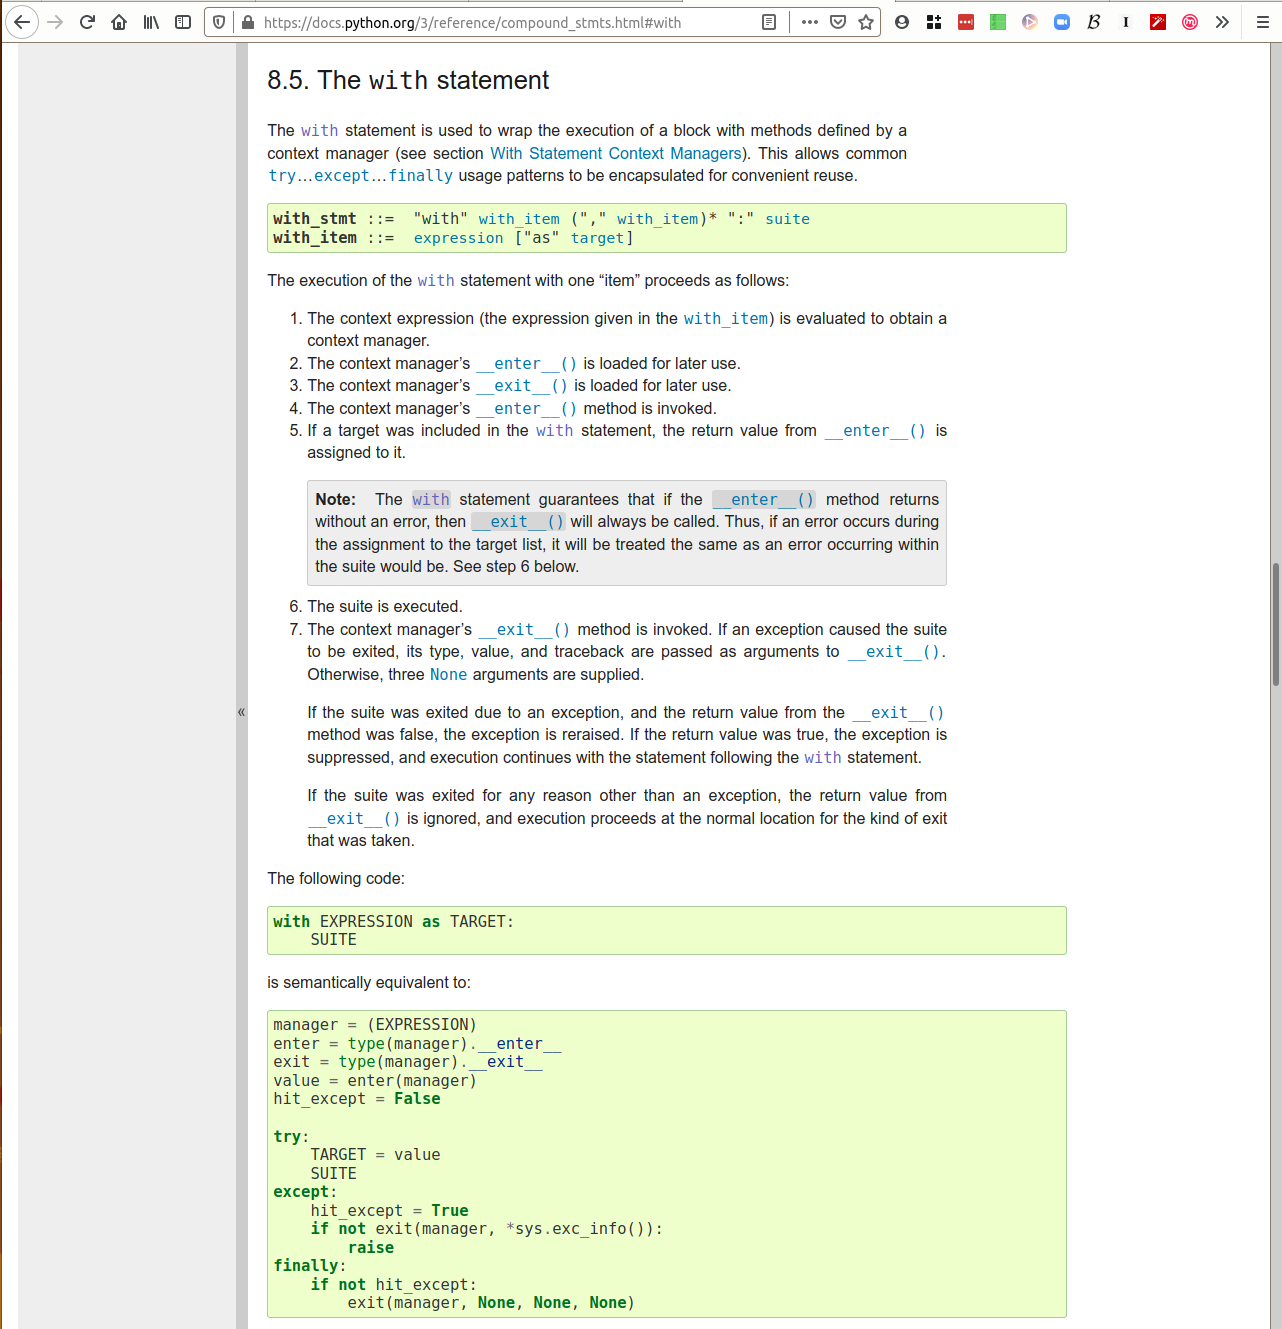
\includegraphics[width=\columnwidth]{figs/docs-with.png}
%\end{frame}

\begin{frame}[fragile]
  \begin{lstlisting}[numbers=none,basicstyle=\Large]
with open("filename", "r") as file:
  print(file.read())
  \end{lstlisting}
\end{frame}

\begin{frame}[fragile]
  \begin{example}[open\textunderscore close.py, del 2]
    \lstinputlisting[linerange=18-28,firstnumber=18]{examples/open_close.py}
  \end{example}
\end{frame}

\subsection{Skriva till filer}

\begin{frame}[fragile]
  \begin{example}[write\textunderscore file.py, del 1]
    \lstinputlisting[linerange=3-10,firstnumber=3]{examples/write_file.py}
  \end{example}
\end{frame}

\begin{frame}[fragile]
  \begin{example}[write\textunderscore file.py, del 2]
    \lstinputlisting[linerange=12-19,firstnumber=12]{examples/write_file.py}
  \end{example}
\end{frame}

\begin{frame}[fragile]
  \begin{example}[write\textunderscore file.py, del 3]
    \lstinputlisting[linerange=20-26,firstnumber=20]{examples/write_file.py}
  \end{example}
\end{frame}

\subsection{Läsa från filer}

\begin{frame}[fragile]
  \begin{example}[read\textunderscore file.py]
    \lstinputlisting[linerange=3-9,firstnumber=3]{examples/read_file.py}
  \end{example}
\end{frame}

\begin{frame}[fragile]
  \begin{example}[read\textunderscore file.py]
    \lstinputlisting[linerange=11-18,firstnumber=11]{examples/read_file.py}
  \end{example}
\end{frame}

\subsection{Typer av filer}

\begin{frame}
  \begin{remark}[Två typer av filer]
    \begin{description}
      \item[Textfiler] Antar \enquote{läsbara tecken}, rader bryts med 
        \lstinline{\\n}.
      \item[Binärfiler] Ingen struktur.
    \end{description}
  \end{remark}
\end{frame}


\section{Filformat}

\begin{frame}[fragile]
  \begin{remark}
    \begin{itemize}
      \item Vi behöver skriva så att vi kan läsa.
    \end{itemize}
  \end{remark}
\end{frame}

\subsection{Enkla filformat}

\begin{frame}[fragile]
  \begin{example}[xy.py]
    \lstinputlisting[linerange=3-10,firstnumber=3]{examples/xy.py}
  \end{example}
\end{frame}

\begin{frame}[fragile]
  \begin{example}[xy.py]
    \lstinputlisting[linerange=12-25,firstnumber=12]{examples/xy.py}
  \end{example}
\end{frame}

\subsection{Mer komplexa}

\begin{frame}
  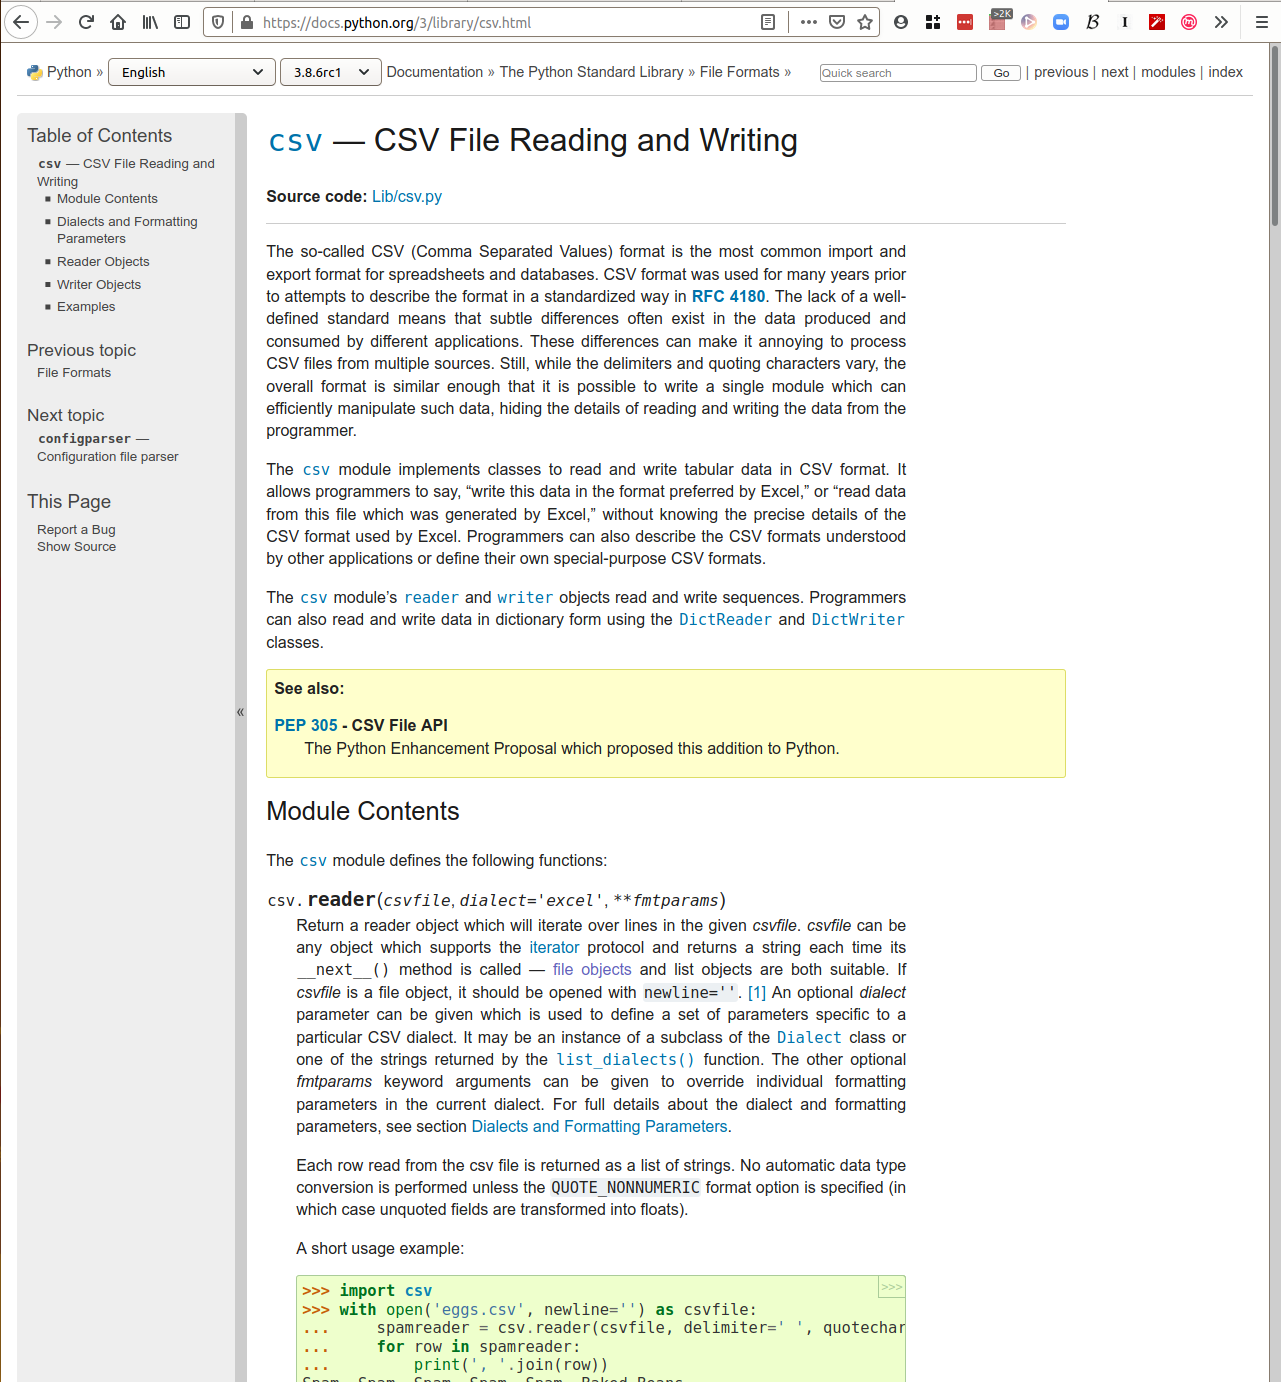
\includegraphics[width=\columnwidth]{figs/docs-csv.png}
\end{frame}

\begin{frame}[fragile]
  \begin{example}[xy\textunderscore csv.py]
    \lstinputlisting[linerange=3-13,firstnumber=3]{examples/xy_csv.py}
  \end{example}
\end{frame}

\begin{frame}[fragile]
  \begin{example}[xy\textunderscore csv.py]
    \lstinputlisting[linerange=15-26,firstnumber=15]{examples/xy_csv.py}
  \end{example}
\end{frame}
